\chapter{D3.js – Data-Driven Documents}
\label{cha:d3js}

Chapter \ref{cha:d3js} provides an overview of the popular JavaScript library D3 which is used to simplify implementations of any data visualizations in the web for developers. The chapter provides an overview of the libraries beginnings but also goes into detail about how to implement projects with D3. The knowledge is required to understand the performance comparisons in chapter \ref{chap:performance} and \ref{chap:conclusion}.

\begin{figure}
    \centering
    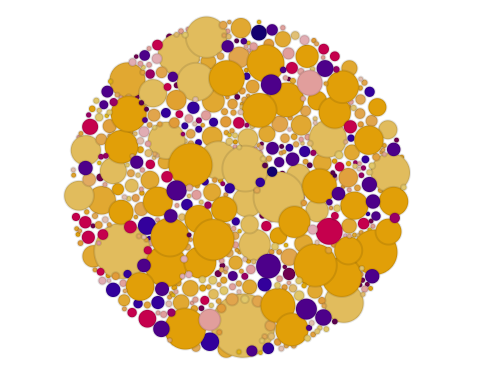
\includegraphics[width=0.5\columnwidth]{force001.PNG}
    \caption{The force graph with default center force. All nodes are attracted to the same center without overlapping each other.}
    \label{fig:force001}
  \end{figure}

\section{Introduction to D3}

D3 is a JavaScript library that helps developers create highly sophisticated data visualizations on the web via a universal tool that is platform agnostic: the browser. The official documentation of D3 in \cite[Introduction]{D3Website} explains the library as a toolkit, that allows binding data to the DOM. Also, it gives an overview of the vast amount of helpful tools that can be used to visualize data. The library includes all kinds of functionality, ranging from picking color ranges, choosing animation springs, randomizing numbers to rendering simple bar charts or calculating treemaps or real-time rendered force simulations.

\begin{figure}
  \centering
  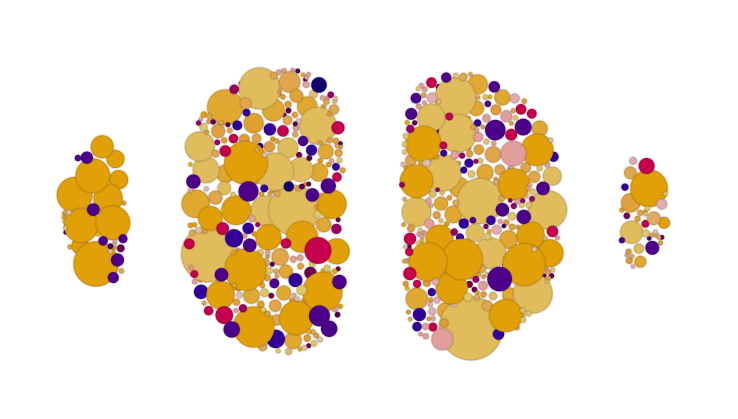
\includegraphics[width=0.6\columnwidth]{force002.PNG}
  \caption{A sample force graph with more than one center force. Having more than one force centers means that different nodes are attracted to their assigned center force.}
  \label{fig:force002}
\end{figure}

\begin{emergency}{1em}
There are multiple examples on the documentation's example page in \cite{D3Examples} which show what developers can achieve by using the D3 library. The API documentation is a comprehensive documentation of the complete feature set of D3 as seen in \cite[\mbox{/d3/blob/master/API.md}]{D3Github}. Due to the immense size of D3, the focus of this thesis and its project lies on a rather ''small'' but quite important part of the library -- the force graph simulation functionality.
\end{emergency}

\section{Force Graphs -- Real time rendered data visualizations}

This paper focuses on a special graph type which is called ''force simulation''. It is the graph type that is integrated into React as showcased by the thesis project. The visualizations consist of objects that interact with each other in a two-dimensional space. By interacting and moving objects all other objects in the animation are also affected. Figures \ref{fig:force001} and \ref{fig:force002} show an example of D3's force simulation. In figure \ref{fig:force001} there is a single center force that keeps all nodes in the center but also keeps individual nodes from overlapping each other. Force graphs can also be configured to make nodes reject each other even further than their actual size as figure \ref{fig:force004} shows. It is also possible to implement so-called links, that also add some complexity to the simulation, as nodes are dependent on each other and not only reject each other but also attract linked nodes as figure \ref{fig:force002} and \ref{fig:force005} shows.

\begin{figure}
    \centering
    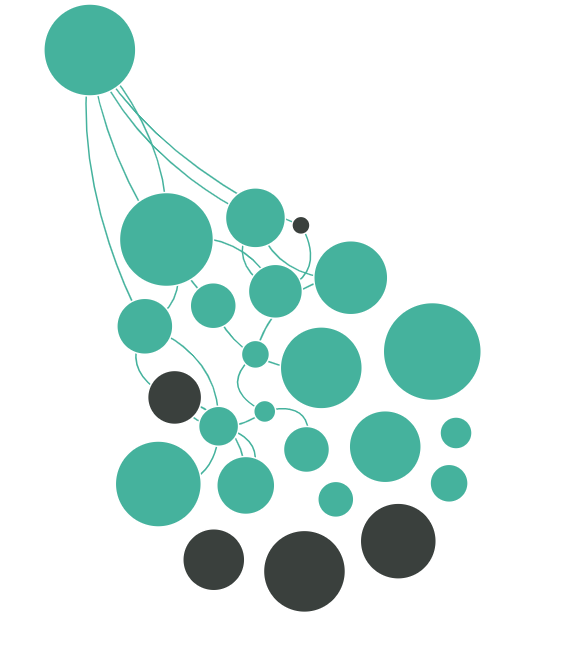
\includegraphics[width=0.4\columnwidth]{forceOwn002.PNG}
    \caption{A sample force graph where the top node is dragged up to the left and the other nodes are dragged along. The force is still keeping the other nodes apart and also drawn to the center though.}
    \label{fig:force003}
  \end{figure}

As previously mentioned, all force simulations are calculated, animated, and rendered in the browser which also includes user interaction. The user can for example drag nodes around which of course then affects other nodes and the whole simulation. Figure \ref{fig:force003} shows well, how dragging one node affects the whole force graph, as all connected nodes follow the dragged node while still rejecting each other and while being attracted to the center force.

D3 provides a somewhat simplified API to be able to quickly implement force graphs in the browser as it can be read in \cite[/d3-force/blob/master/README.md]{D3Github}. The way force simulations work is that developers first have to define or build the simulation. There is a factory method as seen in \hyperref[prog:simulation]{line 1} which takes the nodes of the graph as an argument and builds a default simulation. The nodes have to be provided in a particular scheme so D3 can correctly parse the node array. 

\begin{figure}
  \centering
  
\includegraphics[width=0.45\columnwidth]{forceOwn003.PNG}
  \caption{A sample force graph with one center force. The nodes are configured to reject each other with the function \texttt{r+r/2}}
  \label{fig:force004}
\end{figure}

\begin{program}
\caption{Code snippets for D3 force simulation code}
\label{prog:simulation}
\begin{JsCode}
simulation.forceSimulation([nodes]) // factory method for a standard force simulation
simulation.tick([iterations]) // called on every tick the simulation goes through
simulation.start() // starts a stopped simulation
simulation.stop() // stops a started simulation
simulation.restart() // restarts a simuliation, resets alpha
simulation.alpha([alpha]) // directly sets alpha value
simulation.alphaTarget([alphaTarget]) // sets alpha target value
\end{JsCode}
\end{program}

Another very important aspect of force graphs is the so called ''alpha'' value system as documented in \cite[/d3-force/blob/master/README.md]{D3Github}, which controls how long the simulation lives. The alpha valueis a gradually decaying value that makes the simulation stop if a certain value is reached. Every simulationhas a function that is called every ''tick'' of the simulation as shown in \hyperref[prog:simulation]{line 2}. Everytick the alpha value decays via a predefinable function, it happens logarithmically per default. The tickingfunction takes a handling function will be passed every node position in the simulation which then letsdevelopers link the data to the dom with D3 again. The tick function will be very important lateron when thecombination of D3 and React is explained in more detail.

\begin{figure}
    \centering
    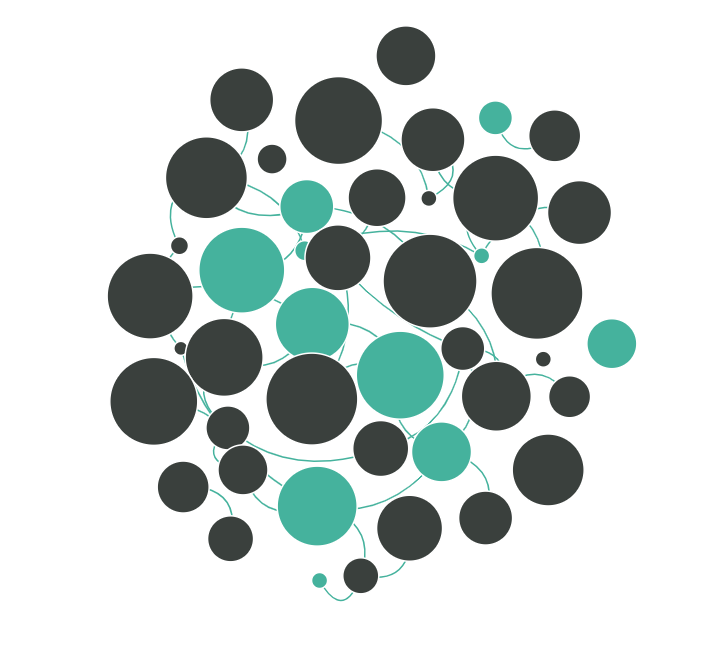
\includegraphics[width=0.45\columnwidth]{forceOwn001.PNG}
    \caption{A sample force graph where some nodes are linked together while still rejecting each other;}
    \label{fig:force005}
  \end{figure}

If there is a user interaction, the simulation sometimes has to be restarted or reheated. Programmers can set alpha values and targets to reheat or restart the simulation in case a node is dragged by the user which would possibly require many other nodes in the simulation to react to that user input. That way also the speed of the simulation can be controlled via setting a custom decay function. The documentation in \cite[/d3-force/blob/master/README.md]{D3Github} points to a few methods that can achieve said functionality. There is for example the functions which can be found in \hyperref[prog:simulation]{line 3}, \hyperref[prog:simulation]{line 4}, and \hyperref[prog:simulation]{line 5} that can be used to reheat a simulation. Also the functions in \hyperref[prog:simulation]{line 6} and \hyperref[prog:simulation]{line 7} values can be set directly to alter the simulation's life span.

%% add code snippets of pure D3

%%\section{History of D3}

%%The library was created in late 2010 according to the documentation in \cite{D3}. 

\section{Explaining the D3 API} 

\begin{program}
\caption{D3 selection, enter, and exit example}
\label{prog:d3selection}
\begin{JsCode}
// earlier in the script

const svg = d3.select('.container')  
const link = svg.selectAll('path')
const node = svg.selectAll('.node')

// handling iterations of the simulation

link.exit().remove()

link = link
  .enter()
  .append('path')
  .attr('stroke', '#45b29d')
  .attr('fill', 'none')
  .attr('id', ({ source: { name: s }, target: { name: t } }) => s + t)
  .merge(link)

node
  .exit()
  .style('fill', '#b26745')
  .transition(t)
  .attr('r', 1e-6)
  .remove()

node
  .transition(t)
  .style('fill', '#3a403d')
  .attr('r', ({ size }) => size)

node = node
  .enter()
  .append('circle')
  .style('fill', '#45b29d')
  .attr('r', ({ size }) => size)
  .attr('id', ({ name }) => name)
  .merge(node)

simulation.nodes(data)
\end{JsCode}
\end{program}

\begin{program}
\caption{Confusing code example}
\label{prog:d3confusing}
\begin{JsCode}
d3.select(_this).classed('active', true)
d3.select(_this)
  .select('.circle')
  .transition(500)
  .attr('stroke', function(d) {
    if (d.rings && d.rings.length > 0) return '#404348'
    return d.color || COLORS[d.type.toUpperCase()] || '#27292c'
  })
  .attr('fill', function(d) {
    return '#404348'
  })
  .style('filter', 'drop-shadow(0 3px 4.7px rgba(0,0,0,.54))')
d3.select(_this)
  .selectAll('.ring')
  .transition(500)
  .attr('opacity', 1)
d3.select(_this)
  .selectAll('.node-background')
  .transition(500)
  .attr('opacity', 0)
d3.select(_this)
  .selectAll('.sub-circle')
  .transition(500)
  .attr('cx', function(d, i) {
    let deg = ((Math.PI * 2) / 8) * i - Math.PI
    let x = Math.sin(deg)
    let offset = event.rings ? event.rings.length * 15 : 0
    return x * (d.r + 5 + offset)
  })
  .attr('cy', (d, i) => {
    let deg = ((Math.PI * 2) / 8) * i - Math.PI
    let y = Math.cos(deg)
    let offset = event.rings ? event.rings.length * 15 : 0
    return y * (d.r + 5 + offset)
  })
  .attr('stroke', '#FFF')
\end{JsCode}
\end{program}

Another very important but general aspect of the D3 API is selecting dom nodes. Via the selection D3 can connect JavaScript data to actual DOM nodes. An example can be seen in \ref{prog:d3selection}. Because the library is not declarative, each node that is added or removed is handled via a chained function call as the append function in the example shows very well. When adding or removing multiple dom nodes (in case the individual nodes of the simulation are complicated dom structures) the code quickly gets very incomprehensive. The provided example only appends one simple circle element for instance. 

The code example \ref{prog:d3confusing} is taken from production code and shows how hard to read D3 code can get if multiple DOM changes have to be handled imperatively. Not only the addition of the nodes has to be handled via function calls, but also the addition of some properties like styles of attributes.

D3 also has the concept of entering and exiting selections. As the code in \ref{prog:d3selection} shows, there are the enter, transition, and exit calls, which only select the nodes which will be new in the current simulation step, which nodes are removed and which nodes are transformed. The chained function calls then can handle those selections accordingly. Again, the provided example is a very simple form of a simulation. If the DOM structure would be more complex, handling any selection would produce confusing and unreadable code very quickly.

According to the documentation in \cite{D3Github} the library D3 was created in 2010. Thus it can be noticed, that the libraries API originates from a time, where developers would not even think about using JavaScript in production. Therefore any code written with D3 is not very scaleable. The example \ref{prog:d3forceinit} shows, that the API is written in a very imperative way. Also the library makes use of a pattern called ''chaining''. The pattern works because each function returns an instance of itself so an infinite amount of functions can be added to the chain, making the code more flexible.

\begin{program}
\caption{Sample initialization of a D3 force graph}
\label{prog:d3forceinit}
\begin{JsCode}
const simulation = forceSimulation(data)
  .force('charge', forceManyBody().strength(-150))
  .force('forceX', forceX().strength(0.1))
  .force('forceY', forceY().strength(0.1))
  .force('center', forceCenter())
  .alphaTarget(1)
  .on('tick', ticked)
\end{JsCode}
\end{program}

Over the year better software patterns have emerged as experience showed, that chaining was a software pattern that was new at the time but can produce code that is hard to maintain. Nowadays this library would probably be written with a functional approach, letting developers compose their own simulations. The problem with the example \ref{prog:d3forceinit} is, that the code cannot be reused, as it is hard coded into the chain. 

\begin{program}
\caption{D3 written in a fictitious functional way}
\label{prog:d3functional}
\begin{JsCode}
const forceParams = compose(
  force('charge', forceManyBody().strength(-150)),
  force('forceX', forceX().strength(0.1)),
  force('forceY', forceY().strength(0.1)),
  force('center', forceCenter()),
)

const simulation = forceSimulation(data)
  forceParams,
  alphaTarget(1),
  on('tick', ticked),
)
\end{JsCode}
\end{program}

If a functional approach would be used the code from \ref{prog:d3forceinit} would look more like in example \ref{prog:d3functional}. One might say, that there is not much of a difference, but actually by looking closer, it is clear, that the variable \texttt{forceParams} is a composition of functions, that can be reused multiple times in the application now. Previously the simulation configuration was locked in the function chain which is a problem that can easily produce duplicated code in any codebase.

%\begin{program}
%\caption{D3 written in a functional way}
%\label{prog:d3foobar}
%\begin{JsCode}
%simulation.foo()
%\end{JsCode}
%\end{program}
%
%Chaining is not the only problem that might decrease the code quality of a project. The other problem of D3 is, %that handling DOM nodes is not declarative but imperative code as well. 
